\documentclass[aspectratio=169]{beamer}

\input{../slides-macros.tex}

\newif\ifmovies%
\moviestrue%
%\moviesfalse

\newif\ifsubs%
\substrue%
%\subsfalse

\newif\ifnotes%
\notestrue%
%\notesfalse

\begin{document}

%======================================================================
\begin{frame}\frametitle{}

\vspace*{0.3in}

\textrm{{\huge\bfseries\color{myOrange} Physics-informed neural networks to solve the compressible Euler equations \\
		\normalsize A parametric hyperparameter tuning approach}}

\vspace*{0.2in}
\hrule

\begin{center}
	\insertmovie{0.49}{animation_1.png}{animation_1.mov}
\end{center}


\hrule

\vspace*{0.1in}
\hfill\cPI{Dario Rodriguez} \rPI{(AE)}\\

\end{frame}
%======================================================================


%======================================================================
\begin{frame}\frametitle{Physics Overview}
	
	\vspace{2mm}
	
	\begin{itemize}
		\item Shock tubes create high-pressure, high-temperature conditions for testing materials, producing combustion
		or as high-pressure gas source in a shock tube-driven wind tunnel
		\item Discontinuities in flowfield arise and experiments are very \textcolor{myOrange}{transitory} in nature (miliseconds) $\rightarrow$ Numerical methods that handle discontinuities (shocks) accurate predictions 
		\item \textcolor{myOrange}{Approach:} conservation laws of mass, momentum and energy (inviscid limit) to characterize the flowfield (\textcolor{myOrange}{Euler equations})  
	\end{itemize}
	
	\vspace{2mm}
	
	\begin{center}
		\insertmovie{0.4}{sod_shock.png}{sod_shock.mov} \\
		\tiny \textit{https://help.sim-flow.com/validation/sod-shock}
	\end{center}

	
\end{frame}
%======================================================================

%======================================================================
\begin{frame}\frametitle{Project Goals}
	
	\textbf{\textcolor{myOrange}{Research question:}} How well a NN can manage \textcolor{myOrange}{irregularities} 
	like shocks? 
	
	\begin{itemize}
		\item Approximate solution of the Euler equations using a neural network using PyTorch
		\vspace{2mm}
		\item Strategies considered: domain extension, weighting losses, clustered sampling of internal points
		\vspace{2mm}
		\item Perform a simple hyperparameter tuning study (trial and error) to set the neural network parameters
		\vspace{2mm}
		\item Compare computational cost with analytical solutions and a classical finite volume method (5\textsuperscript{th} order WENO)
		\vspace{2mm}
		\item \sout{Implement an inverse problem where the physics of a 1-D compressible flow is inferred from
			density gradients data (Schilieren imaging)} 	
	\end{itemize}
\end{frame}
%======================================================================

%======================================================================
\begin{frame}\frametitle{PINNs to approximate high-speed unsteady compressible flows}

Approximate solution of the Euler equations using a neural network and a set of BC/IC
	
	\begin{columns}
		\begin{column}{0.45\textwidth}
			
			\begin{itemize}
				\item 1-D Compressible Euler equations (hyperbolic PDEs in characteristic form)
			\end{itemize}
								 
			\begin{equation*}
				\frac{\partial U}{\partial t} + A \frac{\partial U}{\partial x} = 0
			\end{equation*}
			
			where,			
			\begin{align*}
				U = \left ( \rho, u, p \right)^T \\
				\vspace{10pt}
				A = \begin{bmatrix}
					u & \rho & 0 \\
					0 & u & \frac{1}{\rho} \\
					0 & \rho a^2 & u
				\end{bmatrix} \\
				a = \sqrt{\gamma p / \rho}
			\end{align*}			
		\end{column}
		
		\begin{column}{0.5\textwidth}
		
			\begin{itemize}
				\item \textit{Given} $x$, $t$ $\rightarrow$ \textit{Predict} $\rho$, $u$, $p$
			\end{itemize}
			
			\begin{center}
				\includegraphics[width=0.95\textwidth]{Figures/neural_network_architecture.png}
				\tiny \textit{Mao et al, 2019}
			\end{center}
			
			\textbf{Sod shock tube problem} (Dirichlet BC): 
			\begin{columns}
				\begin{column}{0.5\textwidth}
					\begin{equation*}
						U_L = [1.0, 0.0, 1.0]^T
					\end{equation*}
				\end{column}
								
				\begin{column}{0.5\textwidth}
					\begin{equation*}
						U_R = [0.125, 0.0, 0.1]^T
					\end{equation*}
				\end{column}	
			\end{columns}
			
			
						
		\end{column}
	\end{columns}

\end{frame}
%======================================================================

%======================================================================
\begin{frame}\frametitle{Loss function and training data}
	
	\begin{itemize}
		\item In general, the standard loss function is defined as follows:
	\end{itemize}

	\begin{gather*}
			L(\theta) = \frac{1}{N_f} \left | \frac{\partial \tilde{U}}{\partial t} (x,t,\theta) + \tilde{A} \frac{\partial \tilde{U}}{\partial x} (x, t, \theta) \right |^2_{\Omega \times (0, T],\nu_1} + \\ \frac{1}{N_{IC}} \left | \tilde{U}(x, 0, \theta) - U(x, 0) \right |^2_{\Omega,\nu_2} + \frac{1}{N_{BC}} \left | \tilde{U}(x, t, \theta) - U(x,t) \right |^2_{\partial \Omega \times (0, T],\nu_3}
	\end{gather*}
			
	\begin{itemize}
		\item Since the boundary conditions are induced by the initial conditions, the BC term is dropped, resulting in:
	\end{itemize}
	
	\begin{gather*}
		L(\theta) = L_f (\theta) + L_{IC}(\theta)
	\end{gather*}	

\end{frame}
%======================================================================


%======================================================================
\begin{frame}\frametitle{Training workflow}
	
	Add a diagram that explains:
	\begin{itemize}
		\item Platform used
		\item Data workflow (github, local, remote)
		\item Platform used for development
				
	\end{itemize}
	
	
\end{frame}
%======================================================================


%======================================================================
\begin{frame}\frametitle{Domain Extension and Loss Weighting}
	\begin{itemize}
		\item Domain extends towards the dominant direction of propagation \tiny (Papados, 2021) 
	\end{itemize}
		
	\begin{center}
		\includegraphics[width=0.6\textwidth]{Figures/domain_extension.pdf}
	\end{center}
	
	\begin{itemize}
		\item Loss weighting: $L_f(\theta)$ decreases at a faster rate than $L_{IC}(\theta)$ $\rightarrow$ The NN learns an arbitrary solution to the PDE and tries to adjust it at all interior training points and at all times $(x_n, t_n)$ to fit the IC \tiny (Papados, 2021)
	\end{itemize}
	
	\begin{equation*}
		L(\theta) = w_f L_f (\theta) + w_{IC} L_{IC} (\theta)
	\end{equation*}
	
	
\end{frame}
%======================================================================


%======================================================================
\begin{frame}\frametitle{Uniform and Clustered Sampling}
	\begin{itemize}
		\item A line equation, together with an exponential distribution, were used to randomly sample points near
		the shock location at any time
	\end{itemize}
	
	\begin{center}
		\includegraphics[width=0.9\textwidth]{Figures/points_distribution.pdf}
	\end{center}
	
	
\end{frame}
%======================================================================




%======================================================================
\begin{frame}\frametitle{Results and Analysis}
	
	
\end{frame}
%======================================================================



%======================================================================
\begin{frame}\frametitle{Results and Analysis}
	\begin{itemize}
		\item Domain extends towards the dominant direction of propagation \tiny (Papados, 2021)
		\item  
	\end{itemize}
	
	
\end{frame}
%======================================================================



%======================================================================
\begin{frame}\frametitle{Results - Clustered Sampling}
	
	
\end{frame}
%======================================================================

%======================================================================
\begin{frame}\frametitle{Results - Influence of Neural Network Architecture}
	
	
\end{frame}
%======================================================================

%======================================================================
\begin{frame}\frametitle{Computational cost comparison}
	
	\begin{table}
		\centering
		\begin{tabular}{lc}
			\hline
			Method					& Evaluation time ($T=2$) [s] \\
			\hline
			Analytic				& 			\\
			WENO ($n_x = 100$)		&			\\
			WENO ($n_x = 100$)		& 			\\
			\hline						
		\end{tabular}				
	\end{table}

	
	\begin{table}
		\centering
		\begin{tabular}{lccc}
			\hline
			Case					& Tr/epoch [s] & Tot. Tr. [s] & Eval. ($T=2$) [s] \\
			\hline
			Nominal				&  &  & 			\\
			Ext. Dom		&  &  &			\\
			Loss W.		&  &  & 			\\
			Ext. Dom. + Loss W.		&  &  & 			\\
			E.D. + L.W. + C.S.		&  &  & 			\\
			\hline						
		\end{tabular}				
	\end{table}

	
\end{frame}
%======================================================================

%======================================================================
\begin{frame}\frametitle{Additional Results - Hyperparameter tuning}
	
	
\end{frame}
%======================================================================

%======================================================================
\begin{frame}\frametitle{Results and Analysis}
	
	% Original plot for T=0.1 and T=0.2 for plain NN comparing with WENO and exact
	
	\begin{itemize}
		\item The outcomes from the mentioned trained models are shown below.
		\item A comparison has been made only the exact solution at the desired time ($t=0.2$)
	\end{itemize}
	
	\begin{center}
		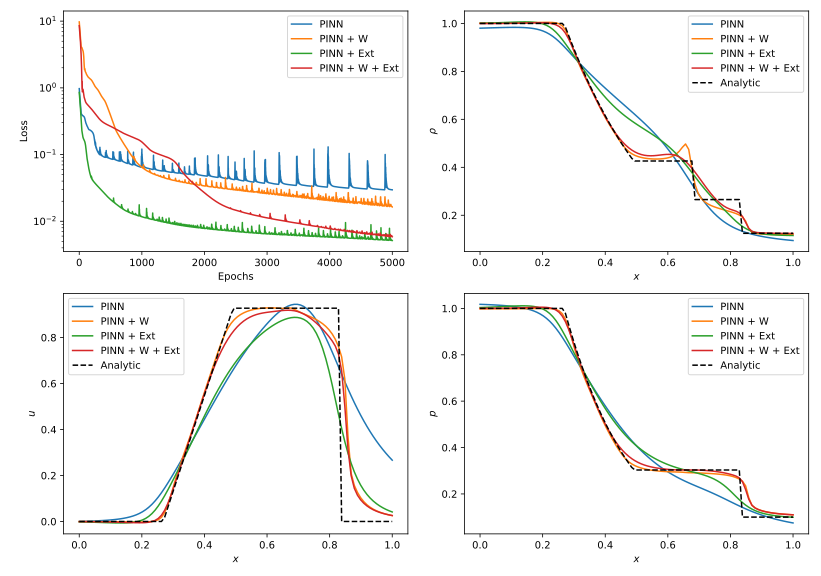
\includegraphics[width=0.65\textwidth]{Figures/preliminary_results.pdf}
	\end{center}
\end{frame}
%======================================================================

%======================================================================
\begin{frame}\frametitle{Summary}
	
	A public repository \includegraphics[width=0.05\textwidth]{Figures/github_logo.png} \alert{\href{https://github.com/dalexa10/Machine_Learning/tree/main/5_Scientific_Machine_Learning/5_PINNs_Euler_Equations}{link}} was setup to host the models implemented
	
	\vspace{3mm}
	
	Four different models were trained by using a neural network (30-neuron width \& 7 hidden layers), a learning rate of 0.0005
	and the classical Adam optimizer. The epochs for these cases were set to 5000
	
	\begin{itemize}
		\item Space domain unaltered ($x \in [0, 1]$), no weights for losses
		\item Space domain extended ($x \in [-1.5, 3.125]$), no weights for losses
		\item Space domain unaltered ($x \in [0, 1]$), loss weights added (0.1 for PDE loss and 10 for IC loss)
		\item Space domain extended ($x \in [-1.5, 3.125]$), loss weights added (0.1 for PDE loss and 10 for IC loss)
	\end{itemize}
	
	
	
\end{frame}
%======================================================================



%======================================================================
\begin{frame}\frametitle{Final Remarks}
	
	\textbf{\textcolor{myOrange}{Conclusions}} 
	\begin{enumerate}
		\item Hyperbolic PDEs highly depend on the initial conditions and its propagation parameters $\rightarrow$ Accuracy of NN increased if this learns the IC first (at higher rate).
		\item In all cases, the accuracy for the velocity and pressure is much higher than that for the density, which is due to the fact the
		velocity and pressure are smooth while the density has a contact discontinuity.
		\item Domain extension and loss weighting demonstrated an improvement in the prediction of the neural network
		\item Clustered sampling showed a better prediction when keeping the NN hyperparameters fixed but it highly depends
		on knowing where the discontinuity located beforehand.
		\item An informal hyperparameter tuning was carried out with no significant improvement in the prediction
	\end{enumerate}
	
	\textbf{\textcolor{myOrange}{Future Work}}
	\begin{itemize}
		\item Add artificial viscosity to rectify the oscillations near shock and contact discontinuities $\rightarrow$ it might
		be really expensive to train the model and it is considered a non-physical adjustment to the mathematical formulation
		\item Impose a \textit{total variation diminishing} condition together with artificial viscosity into the NN  
		
	\end{itemize}
	
\end{frame}
%======================================================================


%======================================================================
\begin{frame}\frametitle{References}
	
	\begin{enumerate}
		\item Mao, Z., Jagtap, A. D., \& Karniadakis, G. E. (2020). Physics-informed neural networks for high-speed flows. Computer Methods in Applied Mechanics and Engineering, 360, 112789
		\item Papados, A. Solving hydrodynamic shock-tube problems using weighted physics-informed neural networks with domain extension.
		\item Michoski, C., Milosavljević, M., Oliver, T., \& Hatch, D. R. (2020). Solving differential equations using deep neural networks. Neurocomputing, 399, 193-212.
	\end{enumerate}
	
\end{frame}
%======================================================================





\end{document}
